\begin{abstract}
A median alert lead time is readily read as a statement about the model: how much warning it
gives. Yet it is also shaped by the cohort, because a first threshold crossing can only be found
within each patient's available pre-onset window. A single median cannot separate model behavior
from the distribution of those windows, making this a reporting problem before it is a modelling
one. That a lead time cannot exceed its search
window is definitional; what has not been measured is how much of a reported number that window
accounts for. Across three perioperative cohorts and five model families, at thresholds
transported unchanged from a development validation split, median lead rises from the shortest
to the longest realized pre-onset window group in all fifteen model-by-cohort combinations, by
26 to 54 minutes. Read beside its operating point, the longest median lead here, 24 minutes,
comes from the combination with the lowest case-level specificity, 0.406. Two natural repairs
leave the dependence in place. This is an empirical measurement-and-reporting case study; we do
not measure what clinicians understand from the term. A median lead remains a descriptive
interval among detected cases, but on its own it does not support a model-intrinsic or
cohort-comparable reading of warning capability. We recommend reporting the pre-onset window
distribution, the operating point, and a window-conditional or explicitly qualified
horizon-specific timing measure beside any single median, and set out four candidate disclosures,
a task-specific complement to TRIPOD+AI.
\end{abstract}

\section{Introduction}\label{introduction}

\textbf{Why a warning interval matters here.} Mean arterial pressure is the average arterial pressure
over one heartbeat, and it is the number an anesthetist watches most closely during an operation.
When it falls below roughly 65 mmHg and stays there the episode is intraoperative hypotension, and
how much a patient accumulates is associated with kidney and myocardial injury after surgery
\citep{walsh2013map, salmasi2017ioh, wesselink2018ioh, sessler2019poqi}. The responses are ordinary
anesthetic care, and none acts the instant it is chosen, so a warning interval is worth something
to the extent that it is time in which a clinician can choose and deliver one. That is why
monitors here are marketed and evaluated on how far ahead they alert \citep{hatib2018hpi, davies2020hpi, wijnberge2020hype, maheshwari2020hpi}. This paper is about that reported interval
and not about physiology: the outcome is defined on mean arterial pressure, which is also a model
input, and Section 4.2 says what that does and does not license.

A model that is read continuously is asked how early it warns, and the \textbf{median alert lead time}
is the statistic reported in answer across acute care: the interval between the first minute a
case's score crosses an alert threshold and the onset of the event. We have not surveyed how often
it is reported, so what follows is a multi-cohort case study rather than a field-level audit. It appears across acute care, for sepsis
\citep{wong2021sepsis}, for acute kidney injury \citep{lee2026aki}, and for intraoperative hypotension,
where a commercial index is marketed on the interval between its alert and the event. The statement
that a system has a \textbf{median alert lead time of 24 minutes} invites the reading that it will
usually give around twenty-four minutes of warning, and that reading is what makes the number worth
reporting. We study the correspondence between the statistic and that invited reading; we do not
measure clinician comprehension directly.

The definition is the same in every one of those settings, and it carries a dependence that
its name conceals. Score every eligible minute, compare against a threshold, and record the
interval between the first crossing and the event. The first crossing is searched for inside
the interval the patient was observed, so the lead is bounded above by the observation
window. The available run-up to onset is set by event timing relative to eligibility, by
monitoring practice and by case mix rather than by the model.

\textbf{What is already known, and what is new here.} Criticism of early-warning evaluation is not
new: the C-statistic has been argued uninformative for early warning scores, with per-alert and
workload measures proposed instead \citep{romerobrufau2015cstatistic}; monitor alerting has been
quantified as a per-hour burden \citep{paine2016alerts}; choice of evaluation sample moves reported
performance for this exact task on these public data \citep{yang2025selection}; and cross-center
evaluation separates learned methods from pressure-derived rules far less cleanly than
single-center reports suggest \citep{chaari2026crosscenter}. That a lead time cannot exceed the window
it is searched in is likewise definitional, and Section 3.3 treats it as such. What is not
established is \textbf{how much of a reported lead time is the window}, and the substitutes those
critiques recommend are what Section 6.2's second item asks for.

\textbf{We make four contributions.} We measure the dependence, in the metric's own units and against
two explicit references rather than against the ceiling (Section 3). We report the operating point
beside the lead, which no lead-time statistic carries, and find the two run opposite to one another
across combinations (Section 4). We implement the two repairs the first two sections invite and
neither works, while a window-conditional statistic that does work disagrees with the median
(Section 5). And we map the case study onto an author-completed TRIPOD+AI
\citep{collins2024tripodai} checklist, which did not request the disclosures that would have made any
of this visible, and propose four candidate additions for continuously monitored models
(Section 6). The argument is about a reported quantity, not about how well any model discriminates,
which is not in dispute here.

\section{Setting}\label{setting}

\textbf{Task and outcome.} Intraoperative hypotension is mean arterial pressure below 65 mmHg sustained
for at least three consecutive minutes, the conventional threshold in this literature
\citep{walsh2013map, salmasi2017ioh, sessler2019poqi}. Mean arterial pressure is also one of the
models' input channels, so the label is computed from a signal the models read; Sections 4.2 and 7
say what that does not license.

\textbf{Cohorts.} Development used MOVER's EPIC arm; we evaluate on its held-out test split (1,404
cases, 786 with a sustained event) and on two external cohorts, VitalDB \citep{lee2022vitaldb, lee2022vitaldbdataset} with 2,804 cases and 1,007 events, and the SIS-derived arm of MOVER
\citep{samad2023mover, samad2023moverdataset} with 2,641 cases and 1,409 events. MOVER (SIS)
releases no usable subject key, so cases are the clustering unit there and subjects in the other
two; all intervals in this paper are 95\% cluster bootstrap on that unit unless a caption says
otherwise.

\textbf{Models.} Five families, spanning the range a clinical team would realistically compare: a
transformer over irregularly sampled triplets \citep{tipirneni2022strats}, referred to throughout as
the ITE Transformer, an LSTM, XGBoost, random forest and logistic regression. Two read the
window as a sequence and three a per-minute feature vector; Appendix A.1 has the architectures
and training. No model is proposed for clinical use and none of what follows is a ranking.

\textbf{Deployment simulation.} Every model is read forward at \textbf{every eligible minute of every
case}, using only measurements recorded strictly before the prediction minute and after a
source-specific exclusion for the induction artifact (Appendix A.1), so a 1,404-case cohort yields
tens of thousands of scored case-minutes from cached data after the fact.

\textbf{Operating points.} An \textbf{operating point} is the score threshold at which the system is read as
alerting, with the sensitivity and specificity that follow. \textbf{Case-level sensitivity} is the share
of event cases that alert at some point in their alert window and \textbf{case-level specificity} the
share of control cases that never do. Calibration and thresholds were fitted on the development
cohort's validation split at an 80\% case-level sensitivity target and then \textbf{transported}
unchanged, applied to every other cohort as fitted rather than re-estimated there. Nothing here
reselects a threshold, split, seed or operating point, and no model is retrained or re-scored.

\textbf{The alert rule and the window it searches.} A case alerts if its score reaches the threshold
at any minute in the 60 minutes before the event, and its lead time is the interval from the
first such minute to the event. The interval the rule searches is the case's \textbf{available
pre-onset evaluation window}: its realized observable run-up to onset, after the induction
exclusion, capped at the 60-minute alert window. A short window is therefore not a briefly or
incompletely monitored case. For an event case it means the event arrived early in the record,
so the run-up \emph{is} the time to onset and there is no missing data to recover. An alert already active at a case's first eligible minute is \textbf{prevalent}; one that
begins later is \textbf{incident}. Cases without an event take a sampled pseudo-onset drawn from the
event cases' timing distribution, so controls are scored over a comparable window. Every lead
time reported here uses this rule unchanged.

\textbf{Ethics.} An institutional review board granted an exemption from review and waived consent for
this secondary analysis (Appendix A.1).

\section{Lead time tracks the available pre-onset window}\label{lead-time-tracks-the-available-pre-onset-window}

\subsection{The number moves with the window, in minutes}\label{the-number-moves-with-the-window-in-minutes}

This section splits detected cases by the length of their available pre-onset window and reads the
median lead separately in each group, which puts the dependence in the metric's own units.

\textbf{The reported lead time moves with the group} (Table A9), the same way in every cell. Median
lead rises from the shortest to the longest realized band in \textbf{15 of 15} model-by-cohort cells,
by \textbf{+26 to +54 minutes}, every interval excluding zero (Table A1), an endpoint contrast of
\textbf{0.51 to 1.02 minutes of lead per minute of window difference}. A single headline figure
therefore describes the cohort's observation-length distribution as much as the model: across
its three cohorts the transformer reports 5 to 9 minutes of median lead for its shortest-observed
band and 46 to 59 for its longest, and the pooled 17 to 24 minutes sits between them because
that is where the median case happens to fall.

\textbf{Detection is itself a function of window length, so we report that rate rather than conditioning
on it silently.} Re-cut on all event cases, the detected share moves with window length in every
cell, by 0.105 to 0.556, falling in the two families that read the window as a sequence and rising
in the three that read a per-minute vector (Table A5). For the transformer the selection runs
\emph{against} the reported gradient, which survives it; for the tabular families it runs with the
gradient, so part of theirs may be survivorship.

\subsection{The same fact as a ratio, in every family}\label{the-same-fact-as-a-ratio-in-every-family}

Section 3.1 gives the dependence in minutes; as a fraction of each case's own window it separates
what is universal here from what is model-dependent.

\textbf{The gradient is universal; its magnitude is not.} The median ratio of a case's lead to its own
observed window is 0.455 to 0.944 and the Spearman correlation between lead and window length is
0.501 to 0.906 across all fifteen cells, again with no interval covering zero. The transformer is the
limiting case at 0.899 to 0.944 with $\rho$ = 0.706 to 0.906, its first alert falling 90 to 94\% of the
way back to the start of the window it was given; the mildest cells are logistic regression in
VitalDB (0.455) and XGBoost in VitalDB (0.467), where the first alert falls closer to the middle
of the window than to its start. The direction holds in every family and cohort while the strength
ranges from near-total to moderate, so a claim that the quantity \emph{is} the window fits the
transformer and overstates the tabular families.

\begin{figure}[H]
  \centering
  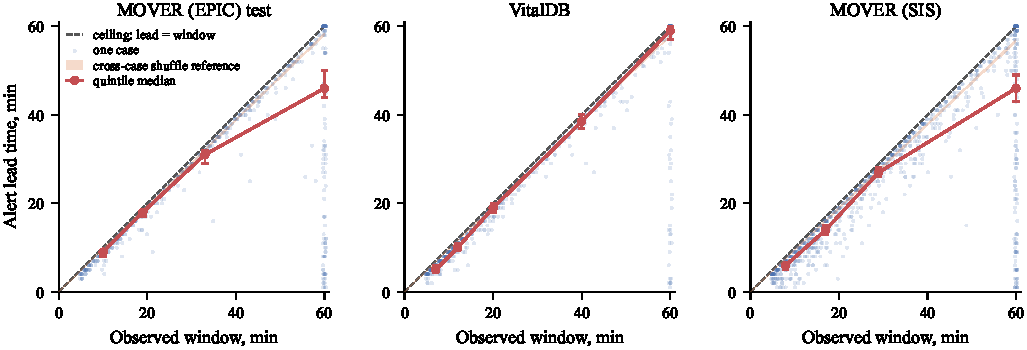
\includegraphics[width=\linewidth]{figures/Figure_2_wide.pdf}
  \caption{\textbf{Alert lead time against the available pre-onset window.} Every detected event case under the ITE Transformer, three held-out cohorts. The dashed diagonal is the ceiling: no crossing can be found outside the case's own window. The shaded band is the 2.5th to 97.5th percentile envelope of the cross-case shuffle reference, not a per-case prediction interval. Red markers are the band medians of Table A9 with 95\% cluster bootstrap intervals; all five families are Figure A1.}
  \label{fig:1}
\end{figure}

\subsection{Explicit references for the ceiling dependence}\label{explicit-references-for-the-ceiling-dependence}

Part of the relationship is built into the definition: a lead time cannot exceed the window it is
searched in, so the ratio is bounded in {[}0, 1{]} by construction and positive dependence can arise
without patient-specific timing. A bound does not specify a distribution, so we use two explicit
references rather than treating the diagonal as a null.

\textbf{The interpretive rule comes before the numbers, because it decides what they can mean.} Both
references are biased \emph{toward} agreement with the observed values, in the direction that favors our
own reading, so each is an upper bound on what a window-only process could produce. A reference
that reaches or exceeds the observed value is therefore the expected and uninformative outcome;
what would be informative is one falling clearly short, and neither does.

\textbf{A continuous uniform reference has median 0.5.} Placing a pseudo-crossing uniformly on each
case's own window gives a reference median of 0.518 to 0.534, which the observed ratio exceeds by
\textbf{+0.372 to +0.421} for the transformer. It does not exceed it everywhere: in \textbf{2 of 15} cells
the observed ratio sits \emph{below} the reference and in one more it is indistinguishable from it, all
three VitalDB cells (Table A2).

\textbf{A cross-case shuffle preserves the aggregate relationship} (Figure 1). Each recipient keeps its
window and reference time but receives another case's whole score sequence, aligned by elapsed
window time, so generic elapsed-time shape survives while the match between trajectory and
recipient is destroyed. Permutations are derangements, 1,000 per cell, so no case keeps its own
sequence. The shuffled median ratio is \textbf{0.72 to 0.97} and
Spearman \textbf{0.63 to 0.94}, so the reference exceeds the observed ratio in \textbf{15 of 15} cells,
which under the rule above is what an upward-biased reference is expected to do. Under a
length-matched variant the observed correlation is \textbf{not distinguishable from the reference in 9
of 15 cells}, and the reference is the larger in 6 of 15 (Table A2).

\textbf{Under these deliberately conservative references the observed association did not exceed what a
window-only reassignment can produce.} That is not the same as showing that a window-only process
generates it, nor that patient-specific information is absent. Reassignment also changes which
event cases are detected, and both variants bias upward, by selecting longer, already-settled
donors or holding a short donor's last value. They bound the dependence rather than estimating a
case-independent process.

\section{Score behavior behind the reported lead}\label{score-behavior-behind-the-reported-lead}

Section 4.1 identifies a direct mechanism for one model. A cross-family property of the score
paths is consistent with it without establishing its cause, and is reported in Appendix A.4
beside Table A3.

\subsection{The transformer is above its own alert threshold almost immediately, in event and control alike}\label{the-transformer-is-above-its-own-alert-threshold-almost-immediately-in-event-and-control-alike}

This section asks what the score is doing at the minutes the alert rule reads, and what the
operating point behind the reported lead looks like.

\textbf{Within one minute of its first scored minute the transformer's median score is already
above the threshold its operating point uses, and it is there for event and control cases
equally} (Figure A5).

In MOVER (EPIC) the median score rises from 0.530 at the first scored minute to 0.938 one
minute later in control cases, and from 0.541 to 0.951 in event cases, against a transported
threshold of \textbf{0.894}. By minute five the two groups are at 0.973 and 0.975, a separation of
0.002 in a score whose scale runs to 1. VitalDB behaves the same way, reaching 0.966 and
0.973. MOVER (SIS) settles more slowly, at 0.833 and 0.906 by minute two and 0.942 and 0.962
by minute five, but it too clears the threshold and it too does so in both groups.

The consequence for the metric is direct. A case whose score settles above the threshold
within its first monitored minutes will register its first crossing as soon as its alert
window opens, whatever else happens, so its lead time is whatever that window holds. That is
the near one-for-one contrast in Table A9.

\textbf{No other family does this} (Figure A5). Sustained elevation is visible in the share of
monitored minutes at or above threshold: \textbf{20.0 to 52.3\% of the transformer's event minutes and
2.5 to 18.3\% of its control minutes, against 0 to 26.7\% and 0 to 1.7\% for the other four
families}.

\textbf{The obvious objection is that this model simply alerts continuously, and reporting the
operating point beside the lead shows that it largely does} (Table 1). Its case-level
specificity is 0.406, 0.379 and 0.467, so it alerts on 53 to 62\% of control cases, and its
positive predictive value of 0.625, 0.380 and 0.585 sits 0.065, 0.021 and 0.051 above the
prevalence it is measured against. This is not a competing explanation of Section 3 but the same
fact: a score above threshold most of the time alerts at the first opportunity, which is what
makes the lead the window. The point is that \textbf{the reported lead carries none of it.} A median
lead of 24, 17 and 22 minutes is the largest of the fifteen combinations and comes from the one
with the least usable operating point.

That holds beyond one model. \textbf{Across the fifteen combinations the reported median lead runs
opposite to case-level specificity} (Spearman $-$0.803, permutation \emph{P} = 0.0008, \emph{q} = 0.006; 86
of 99 untied pairs), and opposite to PPV in excess of prevalence at $-$0.719. Within a cohort the
ordering is 9 of 9 untied pairs in both MOVER cohorts and 8 of 10 in VitalDB, but five
combinations per cohort is thin and none survives adjustment alone, so the pooled figure carries
the claim and cohort confounds it. Two further limits belong with it. The unit is a combination
and not a patient, so these are permutations of the pairing rather than cluster bootstraps. And a
transported threshold does not deliver the same realized sensitivity everywhere: it runs from
0.461 to 0.849 across these combinations (Table A4), so this is a descriptive association among
the operating points as transported, not a sensitivity-matched ranking of models. What it
supports is narrower and still worth stating: a reader ranking these systems by the number they
publish would not be ranking them by how usable their operating points are.

\textbf{Table 1 \textbar{} Case-level operating point behind each reported lead time.} ITE Transformer, three
held-out cohorts, at the transported 80\%-sensitivity operating point every lead time in this paper
uses. \texttt{Min.\ above\ thr.} is the median share of an event case's monitored minutes at or above
threshold. Event prevalence is a property of the cohort, not the cell: 0.560, 0.359 and 0.534.
\textbf{All five families, every interval, the number needed to evaluate, the control-side burden and PPV
in excess of prevalence are Table A4}, where the cross-family claim below is checked.

\begin{longtable}[]{@{}llrrrrr@{}}
\toprule
Model & Cohort & Sens. & Spec. & PPV & Min. above thr. & Lead, min \\
\midrule
\endhead
Transformer & EPIC test & 0.777 & 0.406 & 0.625 & 0.523 & 24 \\
Transformer & VitalDB & 0.679 & 0.379 & 0.380 & 0.444 & 17 \\
Transformer & MOVER SIS & 0.657 & 0.467 & 0.585 & 0.200 & 22 \\
\bottomrule
\end{longtable}

\subsection{What these findings do and do not license}\label{what-these-findings-do-and-do-not-license}

Both findings are properties of a pipeline as deployed with this scoring policy rather than claims
about what any architecture must do; Section 7 states the scope. Neither is a claim about
physiology. The outcome is a sustained excursion of mean arterial pressure and mean arterial
pressure is one of the model's input channels, so the model has direct access to the quantity the
label is computed from, and nothing here shows that a score anticipates a physiological process.

\section{Two natural remedies, and why neither works}\label{two-natural-remedies-and-why-neither-works}

Two fixes follow naturally from Sections 3 and 4, and neither works. A metric with a
plausible-looking repair that fails is a worse problem than one with none, because the repair
gets adopted.

\subsection{Prevalent alerts are not the explanation}\label{prevalent-alerts-are-not-the-explanation}

The first thought is that the metric is dominated by cases already above threshold at their first
eligible minute. Such cases are
\textbf{2.6 to 25.5\%} of detected event cases across
the fifteen cells, and removing them to recompute the median lead on incident alerts alone costs
\textbf{0 to 3 minutes in all fifteen cells}, the transformer included (Appendix A.11).
The relationship of Section 3 is therefore carried by the ordinary cases. Prevalence stays this low
alongside the settling of Section 4.1 because most detected event cases have an available window
shorter than 60 minutes, so it opens while the score is still settling: prevalence and a warm-up
crossing are the same behavior on either side of that minute.

\subsection{Suppressing the first minutes of monitoring is not the fix}\label{suppressing-the-first-minutes-of-monitoring-is-not-the-fix}

The second thought follows from Section 4.1: if the score is unreliable while it settles, discard
alerts raised during that period. We implemented exactly that, discarding every minute at or before
\emph{N} minutes of elapsed monitoring and then applying the unchanged threshold.

At \emph{N} = 5, across all five families and three cohorts, the rule costs \textbf{3.6 to 6.8
percentage points of case-level sensitivity} and returns \textbf{0 to 3.2 percentage points of
specificity}. Median lead changes by \textbf{$-$3 to +1 minutes}; in two of the fifteen cells it
\emph{increases}, because discarding early minutes removes some short-window cases from the detected
set entirely and shifts the median. The trade is poor in every cell, and it does not address
Section 3: the surviving alerts still fire at the first opportunity within whatever window
remains.

The comparison holds the transported threshold fixed, so it is deliberately unmatched on
sensitivity; reselecting a threshold is the one thing this paper does nowhere. The direction is not
expected to reverse under matching: suppression removes alerting minutes and cannot add crossings,
so after lowering the threshold to restore sensitivity, any specificity gain cannot exceed the
fixed-threshold gain above.

\textbf{We therefore do not recommend the rule.} The problem is not that early minutes are noisy.
It is that the reported quantity is coupled to the length of the window it was measured in.

\subsection{What partially helps, and what remains}\label{what-partially-helps-and-what-remains}

Both repairs above change the alert rule and leave the estimand alone. The remaining option
reverses that: condition on window length, or treat the first alert as a time-to-event whose
follow-up ends when the window does, the landmarking treatment of a prediction made at a fixed
point in a run-up \citep{vanhouwelingen2007landmark}. Both are computable from the same cached scores,
so we report them rather than only recommending them (Tables A6 and A7).

\textbf{A horizon-specific detection rate reduces the dependence rather than removing it.} It makes the
horizon explicit and conditions the denominator on event cases observed for at least \emph{X} minutes
before onset. That removes one ambiguity of the pooled median, but window length is still not
constant: cases observed longer than \emph{X} can contribute different amounts of pre-horizon alerting
opportunity. The rate runs 0.278 to 0.692 at a 10-minute horizon and 0.173 to 0.547 at 30 minutes,
declining smoothly with the horizon, a shape a single median suppresses (Table A6).
Restricted instead to cases observed for the whole 60-minute window, so the window is a constant,
the transformer reports the longest median lead of the five families in all three cohorts, 47, 60
and 57 minutes, while detecting only 0.441, 0.247 and 0.304 of them against 0.762 to 0.910 for
XGBoost and the random forest (Table A7): conditioning turns its reported advantage into a deficit.

\textbf{Both remain partial.} The full-window restriction is the stricter window-constant estimand, but
it changes the estimand and the population, discarding 53 to 60\% of event cases: the short-window
cases a deployed monitor will meet. The horizon-specific curve keeps more cases at short horizons
but does not equalize pre-horizon alerting opportunity. Neither repairs the pooled headline median,
and for the reason given in Section 2 the censoring is not independent of the event, with short-
and long-run-up cases differing in surgery duration and case mix (Appendix A.12).

\section{A task-specific reporting extension}\label{a-task-specific-reporting-extension}

Reporting conventions decide what interpretation is available to a reader. A clinician,
policymaker or science writer meets a number and a name, not the scoring policy behind them, so
what a standard asks for bounds what any of them can conclude. That is why auditing one metric is
a communication result and not only a metrology one.

\textbf{This section maps that case study onto what a general standard explicitly asks for.} A
TRIPOD+AI checklist was completed for this work by its own authors, before Sections 3 to 5 were
conducted, and it did not request the disclosures that reveal the dependence. TRIPOD+AI is a
general minimum \textbf{reporting} standard rather than a validity tool, and one author-completed
checklist cannot assess a general framework in either direction. So what follows is a mapping,
and the items in Section 6.2 are task-specific candidate disclosures that complement the standard
rather than correct, invalidate or demonstrate non-adherence to it.

\subsection{The items that were satisfied}\label{the-items-that-were-satisfied}

\textbf{Item 12e, performance measures and rationale}, is where a lead time is declared: it asks
\emph{which} measures were used and \emph{why}, not what else a measure could be responding to. \textbf{Item 23a,
model performance}, asks for performance with uncertainty, and Table 1 satisfies it. So Table 1
is a compliant table in which a 24-minute lead sits beside a specificity of 0.406, with nothing in
either item requiring a reader to put the two together. Four further items came close and missed
(Table A8), and one pattern runs across them: the available pre-onset window distribution is never
requested, and it is the variable the reported lead correlates with at $\rho$ = 0.501 to 0.906.

\textbf{Item 14, model fairness, is the near miss}, and the most instructive item on the list. The
checklist's own fairness answer records that arterial-line placement selects toward longer,
higher-risk operations. The information that observation length is not distributed at random was
therefore \textbf{already disclosed}, filed as a limitation, where it reads as a caveat about which
patients the findings extend to. Nothing in the standard connects it to the timing metric three
tables away.

\subsection{Four candidate disclosures for continuously monitored models}\label{four-candidate-disclosures-for-continuously-monitored-models}

Each is tied to a measurement in this paper, each is computable from artifacts a study of this
kind already produces, and none requires a new experiment. They have not been validated as a
general reporting framework.

\begin{enumerate}
\def\labelenumi{\arabic{enumi}.}
\item
  \textbf{Report alert composition by elapsed observation time}: for every operating point, the share
  of alerts already active at the first eligible minute, those that fired within a short settling
  period, and those that fired later (Figure A2). One stacked bar would have made Section 4.1
  visible on inspection.
\item
  \textbf{Report a window-conditional timing statistic as the primary timing quantity.} A
  horizon-specific detection curve may be added as a secondary disclosure, provided its
  denominator and its remaining dependence on pre-horizon alerting opportunity are stated. Any
  single median should be secondary and stratified by the distribution of available pre-onset
  windows it was measured over: the transformer reports 5 to 9 minutes for its shortest-window
  band and 46 to 59 for its longest, and the pooled 17 to 24 carries neither. Tables A6 and A7
  show the two alternatives; Section 5.3 gives their limits.
\item
  \textbf{Report N(t) beside any event-aligned trajectory.} Here the risk set roughly halves between
  the event and 60 minutes before it (1,404 to 708, 2,804 to 1,433 and 2,641 to 1,374), and the
  cases surviving to the far end are the long-window ones, the same selection that drives
  Section 3. \textbf{The denominator is not cosmetic}: recomputing the same bins on only the cases
  observable back to 60 minutes moves the first bin reaching AUROC 0.70 from 15 minutes in all
  three cohorts to 20, 35 and 20, so the horizon a reader would quote changes by up to twenty
  minutes on a reporting choice alone, and neither curve is the true one (Figure A3).
\item
  \textbf{Report a path-versus-displacement summary for any score read as a trend}, so that a series
  travelling much farther than its net displacement is qualified before it is described as rising
  or falling (Table A3 and Appendix A.4).
\end{enumerate}

The first three are disclosure items in the ordinary TRIPOD sense, naming a quantity that must
appear beside one already required; the fourth is closer to a diagnostic, and we offer it as the
weakest of the four for that reason.

\subsection{What this does and does not generalize to}\label{what-this-does-and-does-not-generalize-to}

The specific artifact does not generalize; its shape does. The shape is a quantity named for what
a clinician would experience,
computed from a window whose length varies across patients and is not reported, under a standard
that requires the quantity and not the window. Any continuously read model evaluated with a
first-crossing statistic over variable available windows is structurally susceptible to this
dependence. Its empirical magnitude has to be measured in each setting, and the four items are the
disclosure that would let a reader see it.

\section{Limitations and scope}\label{limitations-and-scope}

\textbf{Retrospective, and one label.} Every score is computed from cached data after the fact: a
retrospective forward-running simulation, not deployment clearance. The outcome is a sustained
excursion of mean arterial pressure below a fixed level, and both the level and the duration are
conventions we did not vary; the label's dependence on a channel the models read is in Section 4.2.

\textbf{One model fit, one family of operating points, and one draw of the control reference times.}
Models were trained at one seed and thresholds come from one validation split at one sensitivity
target, transported unchanged; a different fit or target could move the composition of Section 5.1,
the magnitudes of Section 3 and the operating points of Table 1, and we varied none of them.
Control cases have no onset, so each is assigned a pseudo-onset sampled once at a fixed seed from
the event cases' timing distribution. \textbf{Every control-side quantity here is conditional on that
one draw}: the case-level specificity and positive predictive value of Table 1, the control-side
minute share, and the cross-combination association of Section 4.1 that rests on them. Its
resampling variability is not propagated into any interval we report. Redrawing the reference
times would require rerunning the complete control-side evaluation pipeline for every model and
cohort, so we report all control-side quantities as conditional on the single pre-specified draw
rather than presenting an unperformed sensitivity analysis.

\textbf{Properties of a pipeline, not of an architecture.} Section 4.1 describes what one model does
under one scoring policy on these cohorts, not what sequence models must do. Section 3's effect is
present in all five families, the ratio running 0.455 to 0.944, with the transformer the limiting
case rather than the exception.

\textbf{The references bias upward.} Both shuffle variants make agreement easier to obtain, in the
direction that favors our own reading, and they change the detected-case set. They bound the
dependence rather than estimating a case-independent process.

\textbf{Communication and reporting claims, and one clinical domain.} We analyze the interpretation
invited by the metric's name, not measured clinician comprehension. The TRIPOD+AI assessment was
author-completed, and the four disclosures were demonstrated here rather than validated across
reporting settings or stakeholder groups. Three cohorts, two health systems and two countries
still give one procedure setting and one monitored variable, so they cannot settle whether
Section 6.2's four items are the right four elsewhere.

